%\documentclass[a4paper]{article}
\usepackage[utf8]{inputenc}
\usepackage[spanish, es-tabla, es-noshorthands]{babel}
\usepackage[table,xcdraw]{xcolor}
\usepackage[a4paper, footnotesep=1.25cm, headheight=1.25cm, top=2.54cm, left=2.54cm, bottom=2.54cm, right=2.54cm]{geometry}
%\geometry{showframe}

%\usepackage{wrapfig}			%Wrap figure in text
\usepackage[export]{adjustbox}	%Move images
\usepackage{changepage}			%Move tables

\usepackage{tikz}
\usepackage{amsmath}
\usepackage{amsfonts}
\usepackage{amssymb}
\usepackage{float}
\usepackage{graphicx}
\usepackage{caption}
\usepackage{subcaption}
\usepackage{multicol}
\usepackage{multirow}
\usepackage{wrapfig}
\setlength{\doublerulesep}{\arrayrulewidth}
\usepackage{booktabs}
\usepackage[numbib, nottoc, notlot, notlof]{tocbibind}

\usepackage{hyperref}
\hypersetup{
    colorlinks=true,
    linkcolor=blue,
    filecolor=magenta,      
    urlcolor=blue,
    citecolor=blue,    
}

%Change Font Size

% #1 = size, #2 = text
\newcommand{\setparagraphsize}[2]{{\fontsize{#1}{6}\selectfont#2 \par}}		%Cambia el size de todo el parrafo
\newcommand{\setlinesize}[2]{{\fontsize{#1}{6}\selectfont#2}}				%Cambia el font de una oración

\newcommand{\note}[1]{
	\begin{center}
		\huge{ \textcolor{red}{#1} }
	\end{center}
}

%FONTS (IMPORTANTE): Compilar en XeLaTex o LuaLaTeX
\usepackage{anyfontsize}	%Font size
\usepackage{fontspec}		%Font type

\usepackage{etoolbox}
\usepackage{todonotes}

\newcommand{\observacion}[2]{  \ifnumequal{1}{#1}{ { \todo[inline,backgroundcolor=red!25,bordercolor=red!100]{\textbf{Observación: #2}} } }{  }  }

\setcounter{topnumber}{2}
\setcounter{bottomnumber}{2}
\setcounter{totalnumber}{4}
\renewcommand{\topfraction}{0.85}
\renewcommand{\bottomfraction}{0.85}
\renewcommand{\textfraction}{0.15}
\renewcommand{\floatpagefraction}{0.8}
\renewcommand{\textfraction}{0.1}
\setlength{\floatsep}{5pt plus 2pt minus 2pt}
\setlength{\textfloatsep}{5pt plus 2pt minus 2pt}
\setlength{\intextsep}{5pt plus 2pt minus 2pt}

\newcommand{\quotes}[1]{``#1''}
\usepackage{array}
\newcolumntype{C}[1]{>{\centering\let\newline\\\arraybackslash\hspace{0pt}}m{#1}}
\usepackage[american]{circuitikz}
\usetikzlibrary{calc}
\usepackage{fancyhdr}
\usepackage{units} 

\graphicspath{{../Control de posición no lineal/}{../Control de fuerza no lineal/}{../Control híbrido no lineal/}{../Referencias/}{../Deducción de modelo/}{../Conclusiones/}}

\pagestyle{fancy}
\fancyhf{}
\lhead{22.99 - Automación Industrial}
\rhead{Lambertucci, Londero B., Maselli, Mechoulam}
\rfoot{Página \thepage}

%Items con bullets y no cuadrados
\renewcommand{\labelitemi}{\textbullet }

%
%\begin{document}

\subsection{Control del ángulo}
\label{sec:ls_angulo}

Se tomó la transferencia de la planta a lazo abierto tomando como salida la posición angular, siendo esta:
\begin{equation*}
	P_t = \frac{6.6667}{(s - 6.763)(s + 6.763)}
	\label{eq:p_t}
\end{equation*}

Separando la transferencia en parte de fase mínima y pasa todo se obtienen las siguientes transferencias:

\begin{multicols}{2}
\begin{equation*}
	P_{tpap} = \frac{s + 6.763}{s - 6.763}
	\label{eq:p_t_pap}
\end{equation*}
\begin{equation*}
	P_{tpmp} = \frac{6.6667}{(s + 6.763)^2}
	\label{eq:p_t_pmp}
\end{equation*}
\end{multicols}

Definiendo la ganancia de lazo $L_t = P_t \cdot C_t$, siendo $C_t$ el controlador, se observan los diagramas de Bode y Nyquist. Iterando y buscando que el controlador sea propio, se obtiene el siguiente modelo:

\begin{equation*}
	C_t = \frac{7.0795 \cdot {10}^5}{P_{tpmp}} \frac{ s + 20 }{s (s + 100)^3}	
\end{equation*}

Con dicha transferencia se obtienen los diagramas presentados en las Figuras (\ref{fig:bode_t}) y (\ref{fig:nyqlog_t}).

\begin{figure}[H]
	\centering
	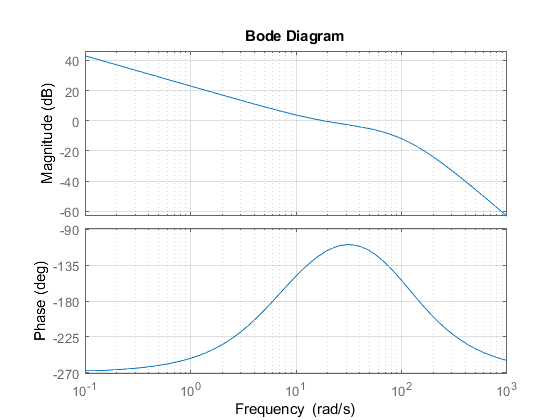
\includegraphics[width=0.6\linewidth]{ImagenesLoop Shaping/Bode_t}
	\caption{Diagrama de Bode de la ganancia de lazo $P_t \cdot C_t$.}	
	\label{fig:bode_t}
\end{figure}
\begin{figure}[H]
	\centering
	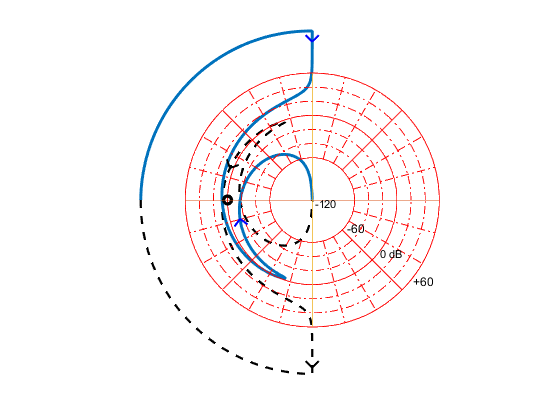
\includegraphics[width=0.6\linewidth]{ImagenesLoop Shaping/Nyqlog_t}
	\caption{Diagrama de Nyquist de la ganancia de lazo $P_t \cdot C_t$.}	
	\label{fig:nyqlog_t}
\end{figure}

\subsection{Control del posición}
\label{sec:ls_pos}

Con lo obtenido en la sección anterior se realiza un subsistema con la planta y el controlador desarrollado.

\begin{figure}[H]
	\centering
	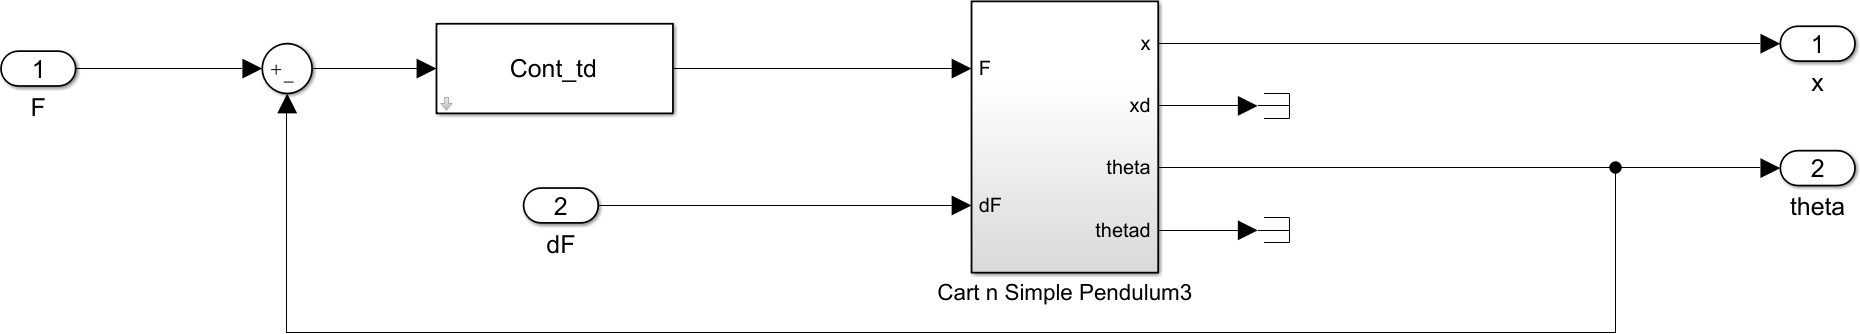
\includegraphics[width=0.6\linewidth]{ImagenesLoop Shaping/ls_t}
	\caption{Control por Loop Shaping del ángulo.}	
	\label{fig:ls_t}
\end{figure}

Linealizando dicho sistema, tomando la posición del carro como salida y con condiciones iniciales nulas, se obtiene la siguiente transferencia:
\begin{equation*}
	P_{x} = \frac{2.1238 \cdot {10}^5 (s+20) (s+6.763)^2 (s+5.718) (s-5.718)}{s^2 (s+183.7) (s+6.766) (s^2 + 8.029 s + 74.89) (s^2 + 101.5 s + 6958)}	
\end{equation*}

Dado que el sistema no pose polo inestables, no se separa el sistema en parte pasa todo y de fase mínima.

De forma análoga a lo realizado en la Sección (\ref{sec:ls_angulo}), se consigue el siguiente modelo de controlador:

\begin{equation*}
	C_{x} = -10.9648 \frac{s + 1}{s + 100}	
\end{equation*}

Se obtuvieron así los diagramas presentados en las Figuras (\ref{fig:bode_x}) y (\ref{fig:nyqlog_x}).

\begin{figure}[H]
	\centering
	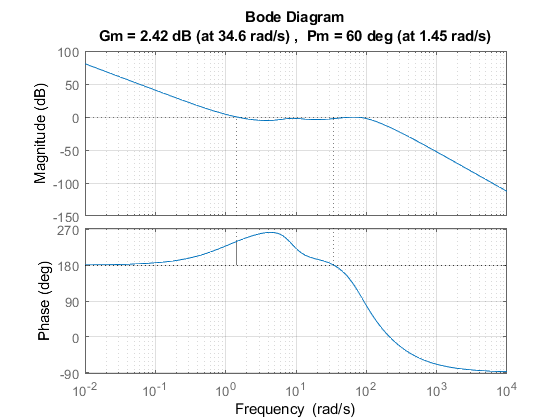
\includegraphics[width=0.8\linewidth]{ImagenesLoop Shaping/Bode_x}
	\caption{Diagrama de Bode de la ganancia de lazo $P_x \cdot C_x$.}	
	\label{fig:bode_x}
\end{figure}
\begin{figure}[H]
	\centering
	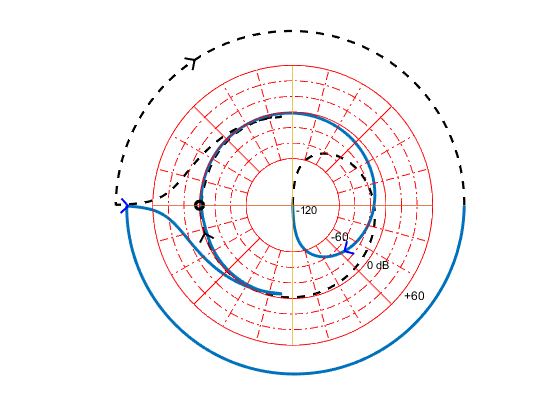
\includegraphics[width=0.7\linewidth]{ImagenesLoop Shaping/Nyqlog_x}
	\caption{Diagrama de Nyquist de la ganancia de lazo $P_x \cdot C_x$.}	
	\label{fig:nyqlog_x}
\end{figure}

\subsection{Control en tiempo discreto}
\label{sec:ls_discreto}

Para conseguir el control en tiempo discreto, se define un período de muestreo $T_s = 1 \ ms$. Además, se consiguen transformar las transferencias $C_t$ y $C_x$ en tiempo discreteo mediante la función \textit{c2d}, siendo estas las siguientes:
\begin{multicols}{2}
\begin{equation*}
	C_{td} = 46.639 \cdot \frac{(z + 1)(z - 0.9933)^2(z - 0.9802)}{(z - 1) (z - 0.9048)^3}
\end{equation*}

\begin{equation*}
	C_{xd} = -10.448 \cdot \frac{z - 0.999}{(z - 0.9048)}
\end{equation*}
\end{multicols}

Colocando bloques de \textit{Zero Order Hold} tanto a la entrada como a las salidas de la planta, se observan las salidas del sistema:
\begin{figure}[H]
	\centering
	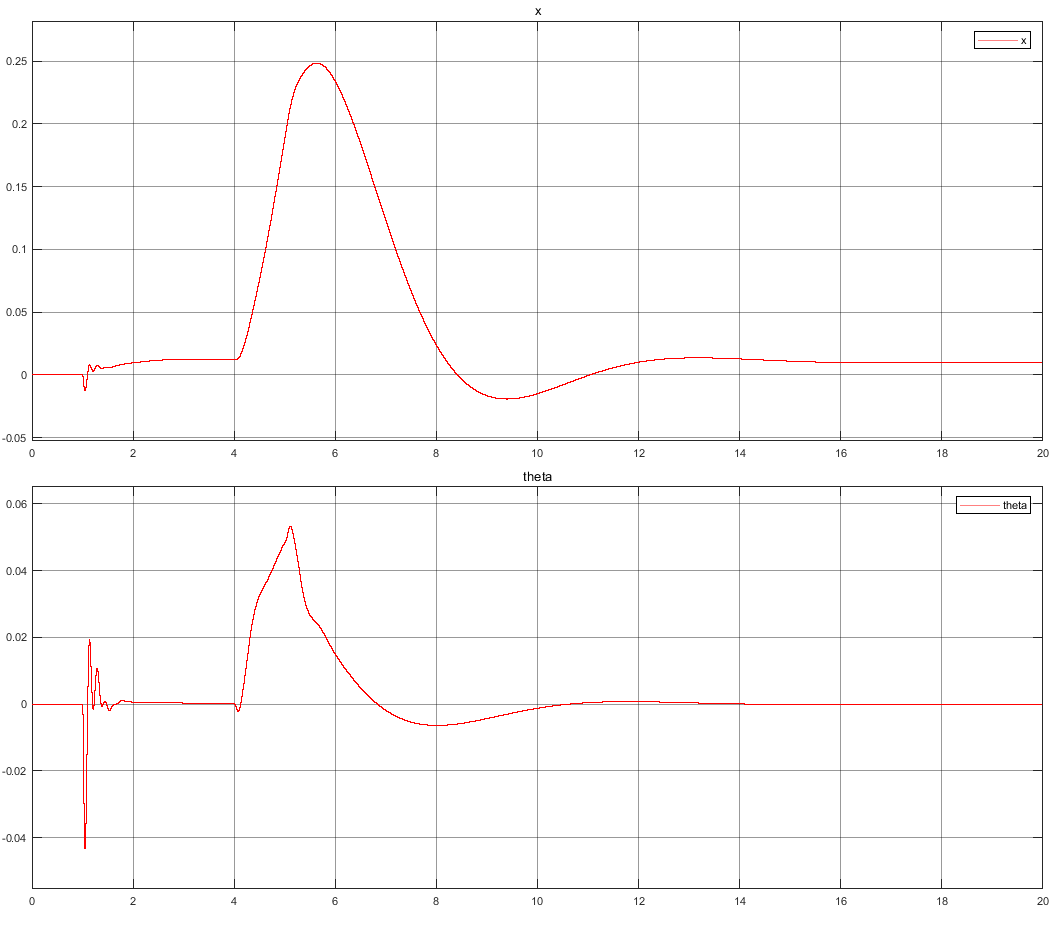
\includegraphics[width=0.9\linewidth]{ImagenesLoop Shaping/salida}
	\caption{Posición del carro y ángulo el péndulo frente a una perturbación.}	
	\label{fig:salida}
\end{figure}


%\end{document}